%% This document is created by 
%%  Dr. Putu Harry Gunawan
%% Template untuk Proposal TA 1 dan TA
%% Template ini digunakan untuk penulisan proposal TA 1 atau TA Fakultas Informatika, Telkom University.

\documentclass[a4paper,12pt,oneside]{book}
\usepackage[utf8]{inputenc}
\usepackage{sectsty}
\usepackage{graphicx}
\usepackage{epstopdf}
\usepackage{algorithm}
\usepackage{algpseudocode}
\usepackage{array}
\usepackage[table]{xcolor}
\usepackage{anysize}
\usepackage{amsmath}
\usepackage{url}
\usepackage{amssymb}
\usepackage[bahasa]{babel}
\usepackage{indentfirst} %Spasi untuk paragraf pertama
\usepackage{geometry}
\marginsize{4cm}{3cm}{3cm}{3cm} %{left}{right}{top}{bottom}
\usepackage[compact]{titlesec} 
\usepackage{etoolbox}

\makeatletter
\patchcmd{\ttlh@hang}{\parindent\z@}{\parindent\z@\leavevmode}{}{}
\patchcmd{\ttlh@hang}{\noindent}{}{}{}
\makeatother

\chapterfont{\centering}
\newcommand{\bigsize}{\fontsize{16pt}{14pt}\selectfont}
\chapterfont{\centering\bigsize\bfseries}
\sectionfont{\large\bfseries}
\usepackage{tikz}
\usetikzlibrary{shapes.geometric, arrows}
\renewcommand{\thechapter}{\Roman{chapter}}
\renewcommand\thesection{\arabic{chapter}.\arabic{section}}
\renewcommand\thesubsection{\thesection.\arabic{subsection}}
\renewcommand{\theequation}{\arabic{chapter}.\arabic{equation}}
\renewcommand{\thefigure}{\arabic{chapter}.\arabic{figure}}
\renewcommand{\thetable}{\arabic{chapter}.\arabic{table}}

\renewcommand\bibname{Daftar Pustaka}
\addto{\captionsbahasa}{\renewcommand{\bibname}{Daftar Pustaka}}
\usepackage{fancyhdr}
\pagestyle{fancy}
\lhead{}
\chead{}
\rhead{}
\lfoot{}
\cfoot{\thepage}
\rfoot{}
\renewcommand{\headrulewidth}{0pt}

\makeatletter

%%%%%%%%%%%%%%%%%%%%%%%%%%%%%%%%%%%%%%%%%%%%%%%%%%%%%%%%%%%%
%
%  Berikut adalah data-data yang wajib diisi oleh mahasiswa
%
%%%%%%%%%%%%%%%%%%%%%%%%%%%%%%%%%%%%%%%%%%%%%%%%%%%%%%%%%%%%

\title{Implementasi \textit{Context-Aware Recommender System} Berbasis \textit{Ontology} untuk Merekomendasikan Tujuan Wisata di Bandung Raya}\let\Title\@title   %Judul dalam bahasa Indonesia

\newcommand{\EngTitle}{Context-aware Recommender System Implementation Based on Ontology for Recommending Tourism Destination at Greater Bandung}  %Judul dalam bahasa Inggris

\author{Rizaldy Hafid Arigi}  \let\Author\@author  %Nama mhs
\newcommand{\NIM}{1103130256}
\newcommand{\Prodi}{Teknik Informatika}
\newcommand{\KK}{Modelling Computational Experiment} %UNTUK TA
\newcommand{\Gelar}{Sains Komputasi} % UNTUK TA
\date{2016}           \let\Date\@date %Maskkan hanya tahun saja
\newcommand{\Tanggal}{11} % Tanggal Pengesahan
\newcommand{\Bulan}{November} % Bulan Pengesahan
\newcommand{\PembimbingSatu}{Z.K. Abdurrahman Baizal, S.Si.,M.Kom}
\newcommand{\NIPPembimbingSatu}{99750047}
\newcommand{\PembimbingDua}{Anisa Herdiani, S.T.,M.T}
\newcommand{\NIPPembimbingDua}{15850002}
\newcommand{\Kaprodi}{Dr. Ketua Program Studi}
\newcommand{\NIPKaprodi}{95650581-1}
\newif\iflogTA
%\logTAtrue   %%%%%% WARNING kode ini diaktifkan untuk format TUGAS AKHIR
              %%%%%% dinonaktifkan jika hanya digunakan untuk Proposal TA 1
\makeatother
\linespread{1}


\begin{document}
\pagenumbering{roman} 
%%\maketitle
\begin{titlepage}
\thispagestyle{empty}
%\vspace*{0.7cm}
{\centering
\large
{\bigsize\bf \Title}\\
\vspace{ 2cm}
\rm
\iflogTA
\textbf{Tugas Akhir}\\
\vspace{0.5 cm}
\textbf{Kelompok Keahlian: \KK}\\
\else
\textbf{Proposal Tugas Akhir}\\
\vspace{0.5 cm}
\textbf{Kelas TA 1}\\
\fi
\vspace{0.5 cm}
\textbf{\Author}\\ \textbf{NIM: \NIM}\\ 

\vspace{1.5 cm}

\begin{figure}[h]
{\centering {
\includegraphics[scale=0.17]{Tel-U-Logo}}\par}
\end{figure}

\vspace{2 cm}
{\bigsize\textbf{Program Studi Sarjana \Prodi}\\
\vspace{0.5 cm}
\textbf{Fakultas Informatika}\\
\vspace{0.5 cm}
\textbf{Universitas Telkom}\\
\vspace{0.5 cm}
\textbf{Bandung}\\
\vspace{0.5 cm}
\textbf{\Date}\\}
}
\pagebreak
\thispagestyle{empty}
{\centering
\iflogTA
\textbf{\large Lembar Pengesahan}\\  %UNTUK TA
\else
\textbf{\large Lembar Persetujuan}\\
\fi
\vspace{0.5cm}
\textbf{\Title}\\
\vspace{0.5cm}
\textbf{\textit{\EngTitle}}\\
\vspace{0.5cm}
\textbf{\Author}\\
\textbf{NIM: \NIM}\\
\vspace{1cm}

\iflogTA 
{ Tugas Akhir ini diterima dan disahkan untuk memenuhi sebagian dari syarat untuk memperoleh gelar sarjana \Gelar\\ Program Studi Sarjana \Prodi\\ Fakultas Informatika Universitas Telkom}\\  %% UNTUK TA
\else
{ Proposal ini diajukan sebagai usulan pembuatan tugas akhir pada\\ Program Studi Sarjana \Prodi\\ Fakultas Informatika Universitas Telkom}\\
\fi
\vspace{0.5cm}

{Bandung, \Tanggal\quad \Bulan \quad \Date}\\
{Menyetujui}\\

\vspace{0.5cm}
\iflogTA
\begin{center}
\begin{tabular}{  m{8cm}  m{8cm} }
Pembimbing 1 & Pembimbing 2
\end{tabular}
\end{center}
\else
\begin{center}
\begin{tabular}{  m{8cm}  m{8cm} }
Calon Pembimbing 1 & Calon Pembimbing 2
\end{tabular}
\end{center}
\fi
\begin{center}
\vspace{2cm}
\begin{tabular}{  m{8cm}  m{8cm} }
\underline{\PembimbingSatu} & \underline{\PembimbingDua} \\ 
NIP: \NIPPembimbingSatu & NIP: \NIPPembimbingDua
\end{tabular}
\end{center}
\vspace{0.5cm}
\iflogTA
Mengesahkan,\\   %% UNTUK TA
Kepala Program Studi \Prodi\\ %% UNTUK TA
\vspace{2.5cm}   %% UNTUK TA
\underline{\Kaprodi}\\ NIP: \NIPKaprodi\\  %% UNTUK TA
\fi
}
\pagebreak
\end{titlepage}
\addcontentsline{toc}{chapter}{Abstrak}
\chapter*{Abstrak}

\par
Sektor pariwisata menunjukkan tren kenaikan untuk sumbangan devisa negara. Salah satu faktor kenaikan tersebut adalah semakin mudahnya mendapatkan informasi tujuan wisata di Indonesia 
melalui layanan Internet yang ada seperti TripAdvisor dan Instagram. Namun hingga saat ini, masih belum ada layanan Internet komersil yang mampu memberikan rekomendasi tujuan wisata 
yang terpersonalisasi. 
\par
\textit{Recommender system} adalah teknik dan kakas perangkat lunak yang digunakan untuk menyediakan rekomendasi item yang sesuai dengan kebutuhan pengguna. 
Untuk dapat menyediakan rekomendasi item sebagai keluaran sistem, tentu dibutuhkan masukan yang sesuai. 
Salah satu teknik yang dapat diterapkan untuk memperoleh masukan \textit{recommender system} adalah \textit{context-aware}. \textit{Recommender system} dapat bersifat \textit{context-aware} dengan memanfaatkan informasi kontekstual pengguna seperti lokasi dan cuaca.
\par
Tugas akhir ini disusun melalui pengembangan dan pengujian \textit{recommender system} yang bersifat \textit{context-aware} dengan 
memanfaatkan masukan berupa lokasi pengguna, cuaca di sekitar tujuan wisata, waktu lokal dan preferensi pengguna terhadap kategori wisata, 
kemudian diproses dengan melakukan \textit{reasoning} pada salah satu model objek dalam \textit{knowledge-based}, yaitu \textit{ontology}, sehingga menghasilkan rekomendasi tujuan wisata.

\vspace{0.5 cm}
\begin{flushleft}
{\textbf{Kata Kunci:} tujuan wisata, \textit{recommender system}, \textit{context-aware}, \textit{knowledge-based}, \textit{ontology}}
\end{flushleft}
\iflogTA
\pagebreak
\addcontentsline{toc}{chapter}{Abstract}
\chapter*{Abstract}

  My abstract here

\vspace{0.5 cm}
\begin{flushleft}
{\textbf{Keywords:} Shallow, water, equations.}
\end{flushleft}
\pagebreak
\addcontentsline{toc}{chapter}{Lembar Persembahan}
\chapter*{Lembar Persembahan}

  Sata persembahkan
  \begin{enumerate}
      \item Kepada Tuhan Yang Maha Esa
      \item Kepada Kedua Orangtua saya
      \item Kepada Rekan kerja dll
  \end{enumerate}
\pagebreak
\addcontentsline{toc}{chapter}{Kata Pengantar}
\chapter*{Kata Pengantar}

\par
Assalamualaikum wr, wb.
\newline
\par
Alhamduillah, puja dan puji syukur saya panjatkan ke hadirat Allah SWT yang telah memberikan rahmat dan
karunia-Nyan sehingga penyusun dapat menyelesaikan tugas akhir dengan judul "\Title".
\par
Dalam tugas akhir ini, penyusun bertujuan untuk mengimplementasikan dan menguji \textit{recommender system}
berbasis \textit{ontology} yang mampu merekomendasikan tujuan wisata dengan memanfaatkan lokasi
pengguna, waktu lokal, cuaca di tujuan wisata dan prefensi pengguna terhadap kategori wisata tertentu
sebagai masukan untuk sistem. Penyusun berharap sistem yang dikembangkan dapat bermanfaat untuk menjadi
sebuah purwarupa untuk \textit{recommender system} yang akan dikembangkan di masa mendatang.
\par
Semoga tugas akhir ini bermanfaat bagi siapapun yang membacanya.

\vspace{2 cm}
\begin{flushright}
Bandung, \today
\\[2cm]
\Author
\end{flushright}
\pagebreak
\fi
\cleardoublepage
\addcontentsline{toc}{chapter}{Daftar Isi}
\tableofcontents
\iflogTA
\newpage
\cleardoublepage
\addcontentsline{toc}{chapter}{Daftar Gambar}
\listoffigures
\newpage
\cleardoublepage
\addcontentsline{toc}{chapter}{Daftar Tabel}
\listoftables
%\pagebreak
\fi
%
\cleardoublepage
\pagenumbering{arabic}
\chapter{Pendahuluan}
\section{Latar Belakang}

Pariwisata telah menjadi sektor ekonomi yang penting di Indonesia. Hal tersebut terbukti ketika pada tahun 2014, sektor pariwisata menyumpang penerimaan devisa negara terbesar
keempat setelah komoditas minyak, batu bara dan kelapa sawit. Pada tahun 2009, sektor pariwisata bahkan menempati peringkat ketiga melebihi batu bara\cite{bps1}. Meskipun memang peringkat penyumbang devisa negara turun, sektor pariwisata berhasil meningkatkan sumbangan devisa dari USD 6,297 miliar di tahun 2010, hingga menjadi USD 11,16613 miliar di tahun 2014 \cite{bps2}.
\par
Pada era teknologi informasi ini, mendapatkan informasi umum apapun yang diinginkan adalah hal yang mudah. Calon turis mencari tahu informasi tujuan wisata secara manual dengan \textit{search engine} atau media sosial merupakan hal yang sudah biasa. Layanan di Internet yang sangat populer untuk mendapatkan rekomendasi tujuan wisata diantaranya TripAdvisor dan Instagram. Namun, mendapatkan informasi tujuan wisata yang sesuai dengan preferensi pengguna melalui cara ini memiliki kelemahan, diantaranya adalah menghasilkan rekomendasi yang kurang terpersonalisasi.
\par 
Rekomendasi yang kurang terpersonalisasi terjadi karena sistem terlalu menitikberatkan pada tujuan wisata yang sangat populer atau sistem tidak tanggap dengan kondisi yang dihadapi pengguna. Untuk mengatasi hal ini, maka \textit{recommender system} yang digunakan harus bersifat \textit{context-aware}\cite{alhazbi2013} dan menggunakan teknik \textit{knowldge-based} untuk memberikan rekomendasi yang adil. Salah satu model representasi pada \textit{knowledge-based} adalah \textit{ontology}. \textit{Ontology} memiliki keunggulan yaitu dapat merepresentasikan informasi kontekstual secara semantik dan kemudahan untuk menjelaskan bagaimana sistem dapat mencapai suatu kesimpulan. Namun, \textit{ontology} sendiri tidak dapat melakukan \textit{reasoning} dengan sendirinya karena \textit{ontology} hanya merepresentasikan pengetahuan. Oleh karena itu dibutuhkan metode \textit{reasoning} untuk mengambil kesimpulan dari representasi pengetahuan yang ada.
\par
Pada prakteknya, \textit{context-aware} cocok untuk diterapkan pada domain pariwisata. \textit{Recommender system} yang bersifat \textit{context-aware} dapat mendukung turis yang sedang bergerak dengan memberikan rekomendasi tujuan wisata yang cocok berdasarkan keadaan lingkungan turis berada dan preferensi turis tersebut\cite{alhazbi2013}. Hal itu dapat dicapai dengan memanfaatkan lokasi pengguna, cuaca dan waktu saat itu \cite{jakkhupan2015}. 
\par
Pada tugas akhir ini akan dilakukan pengembangan dan pengujian \textit{recommender system} dengan teknik \textit{knowldge-based} dan bersifat \textit{context-aware} dengan memanfaatkan variabel lokasi pengguna, cuaca dan waktu serta preferensi kategori wisata yang ingin dikunjungi. Semua variabel masukan tersebut diproses dengan metode \textit{reasoning} berdasarkan model \textit{ontology} yang dibangun dan menghasilkan keluaran berupa rekomendasi tujuan wisata. Pengujian sistem dilakukan dari sisi akurasi rekomendasi dan persepsi pengguna.

\section{Perumusan Masalah}
\begin{enumerate}
	\item Bagaimana model \textit{ontology} yang tepat untuk merepresentasikan pengetahuan sistem pada domain pariwisata?
	\item Bagaimana metode \textit{reasoning} untuk merekomendasikan tujuan wisata?
	\item Bagaimana skema pengujian dari sisi akurasi dan persepsi pengguna untuk \textit{recommender system} yang bersifat \textit{context-aware}?
	
\end{enumerate}
\section{Tujuan Penulisan}
\begin{enumerate}
	\item Membangun model \textit{ontology} yang tepat untuk mereprsentasikan pengetahuan sistem pada domain pariwisata.
	\item Mengimplementasikan metode \textit{reasoning} untuk merekomendasikan tujuan wisata.
	\item Menguji performansi sistem dari sisi akurasi (melibatkan \textit{domain expert}) dan persepsi pengguna.
\end{enumerate}
\section{Batasan Masalah}
\begin{enumerate}
	\item Sistem hanya merekomendasikan tujuan wisata di Bandung Raya, yang meliputi: Kota Bandung, Kabupaten Bandung, Kabupaten Bandung Barat, Kota Cimahi dan Kabupaten Sumedang.
	\item Data masukan hanya berupa lokasi pengguna, cuaca  dan waktu di lokasi pengguna, serta preferensi kategori tujuan wisata pengguna.
	\item Sistem hanya mengeluarkan keluaran berupa rekomendasi tujuan wisata.
	\item \textit{Mobile platform} yang digunakan adalah Android.
	\item Pengguna diasumsikan sedang berada di Bandung Raya ketika menggunakan sistem yang dibangun. 
\end{enumerate}
\section{Rencana Kegiatan}
Kegiatan-kegiatan yang akan dilakukan selama proses penyusunan tugas akhir adalah sebagai berikut:
\begin{enumerate}
	\item Desain sistem
	\par
	Tahap ini menitikberatkan pada perancangan sisi \textit{front-end}, \textit{back-end}, dan representasi \textit{ontology}.
	\item Pengumpulan data lokasi wisata di Bandung.
	\par
	Mengumpulkan data-data wisata di Bandung dengan metode observasi dan wawancara.
	\item Implementasi sistem
	\par
	Mengimplementasikan desain yang telah dibuat pada tahap desain sistem.
	\item Pengujian sistem.
	\par
	Melakukan dua jenis pengujian, satu bertujuan untuk mencari \textit{bug} dan mendapatkan akurasi rekomendasi tujuan wisata dari domain ahli serta sisi 
	persepsi pengguna. 
	\item Pembuatan laporan.
	\par
	Tahap penyusunan laporan berdasarkan kaidah penulisan tugas akhir yang berlaku di institusi.
\end{enumerate}
\section{Jadwal Kegiatan}
Berikut adalah tabel kegiatan dan bulan pelaksanaan.
 
\begin{table}[h!]

\begin{tabular}{||c c c c c c c c||} 
 \hline
 No & Kegiatan & Januari & Februari & Maret & April & Mei & Juni \\ [1ex] 
 \hline\hline
 1 & Desain sistem & \cellcolor{blue!25} & \cellcolor{blue!25} & &&&\\ 
 2 & Pengumpulan data tujuan wisata & & \cellcolor{blue!25} & &&&\\ 
 3 & Implementasi & & \cellcolor{blue!25} & \cellcolor{blue!25} & \cellcolor{blue!25} &&\\
 4 & Pengujian & & & & & \cellcolor{blue!25} &\\
 5 & Pembuatan laporan & & & & & \cellcolor{blue!25} & \cellcolor{blue!25} \\ [1ex]

 \hline
\end{tabular}
\caption{Tabel rencana kegiatan}
\label{table:1}
\end{table}
%
\chapter{Kajian Pustaka}

\section{Wisata dan Pariwisata}
Wisata adalah kegiatan perjalanan yang dilakukan oleh seseorang atau sekelompok orang dengan mengunjungi tempat tertentu untuk tujuan rekreasi, pengembangan pribadi, atau mempelajari
keunikan daya tarik wisata yang dikunjungi dalam jangka waktu sementara.

Pariwisata adalah berbagai macam kegiatan wisata dan didukung berbagai fasilitas serta layanan yang disediakan oleh masyarakat, pengusaha, pemerintah dan Pemerintah Daerah\cite{uupariwisata}.

\section{Recommender System}

\textit{Recommender system} (RS) adalah kakas dan teknik yang digunakan untuk mendapatkan sebuah saran atau rekomendasi item yang dapat digunakan oleh pengguna \cite{ricci2011book}. Rekomendasi item merupakan sebuah keluaran dari proses pembuatan keputusan. Item dapat berupa barang apa yang sebaiknya untuk dibeli, musik apa yang cocok dengan selera pengguna, dan masih banyak lagi.
\par
RS telah banyak digunakan pada media sosial dan layanan-layanan multimedia, contohnya pada Youtube. Youtube adalah sebuah layanan berbagi video milik Google yang sangat populer. RS pada Youtube berperan untuk memberikan rekomendasi video berdasarkan aktivitas pengguna ketika menggunakan Youtube.
\par
Ada tiga teknik yang paling sering digunakan untuk membangun RS, diantaranya adalah \textit{content-based}, \textit{collaborative filtering} dan \textit{knowledge-based}. 
\par
Pada \textit{content-based} RS belajar untuk menghasilkan rekomendasi item kepada pengguna berdasarkan apa yang pengguna sukai sebelumnya\cite{moreno2013sigtur}. Ciri item akan dibandingkan dan dihitung untuk mengetahui asosiasi antar item. Contohnya jika pengguna memberi respon suka pada beberapa video mengenai komputer, maka RS akan memberikan rekomendasi berupa video yang berbicara mengenai pemrograman komputer.
\par
Sedikit berbeda dengan \textit{content-based}, \textit{collaborative filtering} akan menghasilkan rekomendasi item kepada pengguna aktif berdasarkan apa yang pengguna lain sukai sebelumnya yang memiliki selera sama dengan pengguna aktif tersebut\cite{castillo2008samap}. Kemiripan selera dihitung berdasarkan kemiripan histori antar pengguna.
Kedua pendekatan yang telah disebutkan memiliki kelemahan. Permasalahan teknik \textit{content-based} adalah \textit{cold start} dan \textit{overspecialization}. \textit{cold start} muncul ketika pengguna baru aktif di sistem dan RS belum memiliki data mengenai preferensi pengguna. Sedangkan \textit{overspecialization} adalah masalah ketika RS memberi rekomendasi yang kemiripannya terlalu dekat dengan item sebelumnya yang disukai pengguna\cite{blanco2008flexible}. \textit{Collaborative filtering} juga memiliki permasalahan \textit{cold start}\cite{ricci2011book}. Permasalahan \textit{cold start} dan \textit{overspecialization} tidak dimiliki oleh \textit{knowledge-based}.
\par
\textit{Knowledge-based} adalah teknik RS yang merekomendasikan suatu item berdasarkan suatu representasi pengetahuan bagaimana ciri item bisa memenuhi kebutuhan dan selera pengguna serta tingkat kegunaan item untuk pengguna. \textit{Knowledge-based}  menggunakan fungsi kesamaan yang mengestimasi seberapa cocok kebutuhan pengguna dengan rekomendasi yang akan diberikan tanpa memerlukan data histori apapun dari pengguna sehingga masalah \textit{cold start} dan \textit{over-specialization} tidak akan muncul. Selain tidak membutuhkan data histori, \textit{knowledge-based} cocok untuk digunakan untuk pengembangan RS berdasarkan kasus dunia nyata.

\section{Context-aware}

Dalam bidang \textit{ubiqiotous computing}, konteks merupakan lokasi pengguna, identitas orang-orang disekitar pengguna, objek disekitarnya dan perubahan pada elemen-elemen tersebut \cite{ricci2011book}. Informasi kontekstual adalah hal yang sangat vital dalam perolehan rekomendasi yang relevan. Hal tersebut menjadikan \textit{context-aware} merupakan salah satu pendekatan yang efektif dalam memahami kebutuhan pengguna.

Pendekatan penggunaan informasi kontekstual untuk proses rekomendasi dapat dikategorikan menjadi dua kelompok, yang pertama adalah rekomendasi yang menggunakan \textit{context-driven querying} dan yang kedua adalah \textit{contextual preference elicitation and estimation}\cite{ricci2011book}. Pendekatan pertama telah digunakan pada RS untuk pariwisata dan perangkat \textit{mobile}. Sistem menggunakan pendekatan ini untuk mengekstrak informasi kontekstual langsung dari pengguna \cite{van2004context}\cite{abowd1997cyberguide}, contohnya dengan memberi pertanyaan bagaimana suasana hati pengguna saat ini, atau berdasar informasi lingkungan pengguna seperti lokasi, cuaca dan waktu untuk melakukan eksekusi \textit{query} dan mendapatkan item yang paling cocok dengan pengguna. Sedangkan pendekatan kedua memodelkan dan mempelajari preferensi pengguna dengan \textit{collaborative filtering}, \textit{content-based}, atau teknik analisis data dari \textit{machine learning}. Pada RS yang penyusun akan kembangkan, RS menggunakan pendekatan pertama karena pendekatan pertama cocok untuk RS dengan paradigma \textit{knowledge-based} \cite{ricci2011book} dan kompleksitas komputasi yang lebih kecil dari pendketan kedua.

\section{Semantic Web dan Ontology}

\textit{World Wide Web Consortium} (W3C) mendefinisikan \textit{semantic web} sebagai kerangka kerja umum yang dapat memperkenankan data untuk bisa diberikan dan digunakan ulang di lintas aplikasi, perusahaan dan batasan komunitas. Secara khusus, teknologi \textit{semantic web} menawarkan kemampuan menghubungkan data pada sebuah jaringan.
\par
\textit{Ontology} merupakan salah satu bagian penting dalam domain \textit{semantic web}. \textit{Ontology} adalah sebuah cara formal untuk merepresentasikan jaringan taksonomi dan klasifikasi serta mendefinisikan struktur pengetahuan. Pada tugas akhir ini, \textit{ontology} akan digunakan untuk merepresentasikan pengetahuan kategori wisata. \textit{Ontology} akan diimplementasikan dengan menggunakan bahasa khusus untuk membangun \textit{ontology} yaitu \textit{Web Ontology Language} (OWL).
\par
Beberapa penelitian telah mengajukan suatu metode untuk merekonstruksi \textit{ontology}. Salah satunya adalah \textit{Methontology}\cite{jones1998methodologies}. 
Berikut adalah tahap pengembangan \textit{ontology}\cite{fernandez1997methontology}:
\begin{enumerate}
	\item \textit{Planning}
		\par Merencanakan bagaimana suatu tugas (untuk langkah selanjutnya) dilakukan. Hal ini meliputi orang-orang yang terlibat, perangkat lunak dan perangkat keras.
	\item \textit{Spesification} 
		\par Mengidentifikasi tujuan \textit{ontology}, ruang lingkup \textit{ontology}, termasuk istilah didalamnya. keluaran dari tahap ini adalah spesifikasi \textit{ontology} dalam bahasa manusia.
	\item \textit{Knowledge Acquisition}
		\par Wawancara dengan ahli atau studi pustaka pada ruang lingkup terkait dapat membantu akuisisi pengetahuan secara signifikan.
	\item \textit{Conceptualization}  
		\par Data kunci pada suatu domain seperti konsep, \textit{instance}, relasi kata kerja, sifat direpresentasikan secara informal (bahasa manusia).
	\item \textit{Formalization}
		\par Formalisasi dari konsep yang telah dibangun dalam bahasa manusia menjadi konsep formal yang bisa diimplementasikan pada perangkat lunak.
	\item \textit{Integration} 
		\par Tahap untuk menentukan apakah \textit{ontology} lain yang sudah ada dapat diintegrasikan dengan \textit{ontology} yang dibangun.
	\item {Implementation} 
		\par \textit{ontology} direpresentasikan secara formal pada bahasa tertentu, contohnya OWL. 
	\item \textit{Evaluation} 
		\par Tahap untuk mencari definisi yang salah pada \textit{ontology} yang dibangun.
	\item \textit{Documentation}
	\item \textit{Maintenance}
\end{enumerate}

\par
Gambar 2.1 memvisualisasikan tahap-tahap yang dijabarkan diatas.
\begin{figure}[h!]
    \centering
    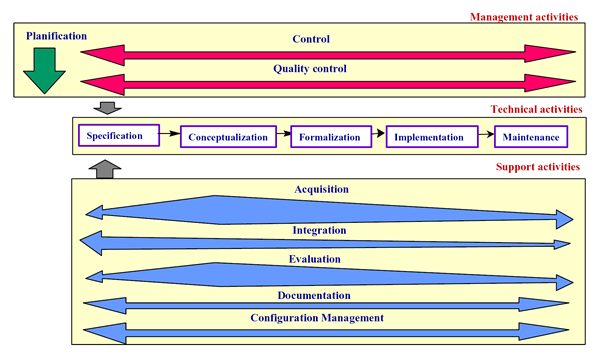
\includegraphics[scale=0.5]{img/methontology_cycle.png}
    \caption{Gambaran tahap-tahap \textit{methontology}}
    \label{fig:Gambar}
\end{figure}

\section{Android}
Android adalah sistem operasi untuk perangkat \textit{mobile} yang dikembangkan oleh Google dengan memanfaatkan \textit{kernel} dari sistem operasi Linux. Sistem operasi ini telah banyak digunakan pada \textit{smartphone}, tablet pc, TV, \textit{wearable device}, dan masih banyak lagi.

Android digunakan sebagai \textit{platform} untuk sisi \textit{front-end} karena kemudahan Android untuk mendapatkan data lokasi pengguna dibandingkan dengan menggunakan PC.

\section{Google Maps API}
Google Maps API \textit{(Application Programming Interface)} adalah sebuah \textit{interface} khusus yang dapat digunakan pengembang perangkat lunak sehingga aplikasi yang dikembangkan dapat menggunakan layanan,fitur dan basis data pada Google Maps.
\par
Google Maps API dipilih karena kemudahan integrasi API pada pengembangan aplikasi Android.  

\section{OpenWeatherMap API}
OpenWeatherMap adalah sebuah API yang menyediakan layanan untuk mendapatkan data cuaca terkini. OpenWeatherMap API memiliki dukungan untuk berbagai macam \textit{platform} seperti Android dan iOS.
\par
Pada tugas akhir ini, OpenWeatherMap akan digunakan untuk mendapatkan data cuaca terkini di lokasi pengguna.

\section{Jython}
Jython merupakan bahasa pemrograman Python yang terintegrasi dengan Java. Berbeda dengan Python biasa yang berjalan dengan \textit{C compiler}, Jython berjalan dengan menggunakan
Java Virtual Machine (JVM). 

\section{Protokol HTTP}
\textit{Hypertext Transfer Protocol} (HTTP) adalah protokol aplikasi yang menjadi dasar komunikasi data pada \textit{World Wide Web}. \textit{Hypertext} adalah teks dengan struktur tertentu yang dikirim diantara \textit{node}. HTTP menjadi protokol agar bisa mengirim \textit{Hypertext}.
\par
HTTP berfungsi untuk memfasilitasi permintaan dan respon data pada model \textit{client-server}. Pada contoh dunia nyata, \textit{web browser} berperan sebagai \textit{client} dengan mengirimkan pesan permintaan HTTP ke \textit{server} yang berperan untuk \textit{hosting}. \textit{Server} akan menyediakan sumber daya yang disebutkan berdasar permintaan HTTP yang diterima dan mengirim respon HTTP kepada \textit{client}.
\par
HTTP memiliki beberapa metode permintaan seperti \textit{GET}, \textit{POST}, \textit{DELETE}, \textit{CONNECT} dan \textit{TRACE}. Metode permintaan yang paling sering digunakan adalah \textit{GET} dan \textit{POST}. Pesan yang dikirim dalam permintaan berisi baris permintaan, \textit{header} dan badan pesan (opsional). Sedangkan respon yang dikirim dengan HTTP berupa kode status permintaan, \textit{header}, dan badan pesan.
\par
Tugas akhir ini menggunakan HTTP sebagai perantara pertukaran pesan antara ponsel pengguna dengan proses yang berjalan pada \textit{server}. HTTP dipilih karena HTTP dapat mengirim pesan dalam berbagai tipe konten seperti teks biasa, html, atau Javascript Object Notation (JSON).   

\section{Javascript Object Notation}
\textit{Javascript Object Notation} atau yang biasa disebut JSON adalah sebuah format pertukaran data. JSON memiliki kelebihan dapat dipahami manusia dengan mudah dan kemudahan \textit{parsing} oleh mesin. 
\newline
Tugas akhir ini menggunakan JSON sebagai format pertukaran data antara \textit{client} dan \textit{web server}.

\section{SPARQL}
SPARQL adalah bahasa \textit{query} untuk basis data \textit{semantic}. SPARQL memiliki kapabilitas membaca dan memanipulasi data yang tersimpan dalam format \textit{Resource Description Framework}(RDF). Data dalam format RDF direpresentasikan dalam bentuk graf. Meskipun begitu, data RDF dapat dikategorikan sebagai database relasional SQL yang menggunakan tiga kolom yaitu subjek, predikat dan objek.
SPARQL akan digunakan untuk menyimpan data \textit{ontology} yang merepresentasikan pegetahuan sistem mengenai lokasi pariwisata Bandung. 
 
%
\chapter{Metodologi dan Desain Sistem}

\section{Pengembangan Ontology}
Dari sepuluh tahap \textit{Methontology}, terdapat tiga tahap utama yang menghasilkan keluaran formal 
yaitu \textit{specification}, \textit{conceptualization} dan \textit{implementation}.
\par

\subsection{\textit{Specification}}
Dalam tahap \textit{specification} pengembangan \textit{ontology}, terdapat tiga hal utama yang yang harus dideskripsikan yaitu domain, tujuan dan lingkup \textit{ontology}
yang dikembangkan.
\par
Tahap ini akan menghasilkan dokumen spesifikasi kebutuhan \textit{ontology} pada domain pariwisata. Tabel \ref{table:ont-spec} adalah spesifikasi dari \textit{ontology} yang akan dibangun.

\begin{table}[h]
\begin{center}
\begin{tabular}{ |l|m{12cm}| } 
\hline
	Domain & Pariwisata \\
	\hline
	Tujuan & Ontology untuk merepresentasikan pengetahuan klasifikasi tujuan wisata dan aktivitas yang dapat dilakukan\\
	\hline
	Lingkup & Daftar kategori tujuan wisata, daftar tingkat kedekatan suatu tujuan wisata dengan kategori tujuan wisata, daftar kategori cuaca, daftar tujuan wisata,
	daftar atribut tujuan wisata. \\ 
	\hline
	Sumber & Wawancara dengan pakar. \newline 
	buku \textit{Tourism Planning, An Integrated and Sustainable Development Approach} karya Edward Inskeep. \\
	\hline
\end{tabular}
\end{center}
\caption{Tabel spesifikasi kebutuhan ontology yang akan dibangun}
\label{table:ont-spec}
\end{table}

Domain dari \textit{ontology} yang akan dikembangkan berada di domain pariwisata, meliputi daya tarik wisata wisata dan kategorinya. Untuk bisa mengetahui bagaimana daya tarik wisata dikategorikan,
maka perlu adanya konsultasi dengan pakar terkait dan studi pustaka pada buku rujukan yang direkomendasikan oleh pakar.

\subsection{\textit{Conceptualization}}
Ketika tahap \textit{specification} telah selesai, maka akan didapat spesifikasi komponen \textit{ontology} (kelas,textit{instance}, atribut, relasi) apa saja yang harus tersedia dan bagaimana
teknik mengakuisisi pengetahuan terhadap komponen tersebut. Pada tahap \textit{conceptualization}, teknik-teknik untuk mengakuisisi pengetahuan diaplikasikan
untuk mendapatkan istilah-istilah pada domain kategori pariwisata. Tabel \ref{table:concept-table} adalah tabel istilah preferensi kategori pariwisata.

\begin{center}
\begin{longtable}{ |l|m{10cm}| } 
\hline
	\textbf{Istilah} & \textbf{Keterangan} \\
	
	\hline
	Daya tarik & Sebuah tempat yang dikunjungi oleh seseorang dengan harapan kebutuhannya yang terkait dengan mengisi waktu luang akan terpenuhi
	\cite{inskeep1991tourism}. Klasifikasi secara umum membagi daya tarik menjadi tiga yaitu alam, budaya dan buatan.\\
	\hline
	Aksesibilitas & Sarana dan infrastruktur penunjang suatu aspek pada daya tarik / daya tarik wisata, contohnya jalan dan listrik.\\
	\hline
	Daya tarik alam & Daya tarik wisata yang ada karena terbentuk secara alami.\\ 
	\hline
	Daya tarik budaya & Daya tarik wisata yang ada karena aktivitas dan kebiasaan manusia.\\
	\hline
	Daya tarik buatan & Daya tarik wisata yang ada karena dibangun oleh manusia.\\
	\hline
	Petualangan alam & Subkelas dari daya tarik alam. Fenomena alam yang tidak biasa seperti geyser, gua, pemandian air panas, aktivitas gunung
	merapi merupakan daya tarik wisata yang penting untuk wisatawan yang ingin melihat-lihat atau melakukan aktivitas khusus seperti
	mendaki dan menjelajah gua. Pada kateogori ini terdapat subkategori \textbf{pemandian air panas}, \textbf{eksplorasi}, 
	\textbf{pemandangan alam} dan \textbf{pendakian}.\\
	\hline
	Flora dan fauna & Subkelas dari daya tarik alam. Konservasi hewan dan tumbuhan yang berada di habitatnya merupakan daya tarik wisata yang
	sangat menarik. Pada kategori ini terdapat subkategori \textbf{konservasi} dan \textbf{safari}.\\
	\hline
	Keindahan alam & Subkelas dari daya tarik alam. Merupakan motivasi utama dalam mengunjungi daya tarik alam. Pada kategori ini terdapat sub 
	kategori \textbf{\textit{camping}}, \textbf{\textit{hiking}}, \textbf{\textit{outbound}} dan \textbf{pemandangan alam}.\\
	\hline
	Pesisir dan perairan & Subkelas dari daya tarik alam. Sungai, danau dan area laut dapat menjadi daya tarik wisata untuk berbagai
	macam aktivitas dari mulai rekreasi hingga olahraga yang menantang seperti \textit{diving} dan \textit{rafting}. Pada kategori ini
	terdapat subkategori \textbf{olahraga akuatik}, \textbf{relaksasi akuatik} dan \textbf{pemandangan alam}.\\
	\hline
	Hiburan & Subkelas dari daya tarik buatan. Kategori hiburan diasosiasikan dengan seni pertunjukan kontemporer dan musik. Klub malam,
	karaoke dan kafe yang menyajikan musik masuk dalam kategori ini. Pada kategori ini terdapat subkategori 
	\textbf{hiburan malam}, dan \textbf{seni pertunjukan}. \\
	\hline
	Event & Subkelas dari daya tarik buatan. Bangunan konferensi yang dapat digunakan untuk mengadakan acara besar seperti konser dan \textit{event}
	merupakan daya tarik wisata yang semakin populer di seluruh dunia. Pada kategori ini terdapat subkategori \textbf{konferensi} dan \textbf{stadion}.\\
	\hline
	Kuliner & Subkelas dari daya tarik buatan. Pada kategori ini terdapat subkategori \textbf{kuliner umum} dan \textbf{kuliner khas}.\\
	\hline
	Olahraga & Subkelas dari daya tarik buatan.Fasilitas rekreasi dan olahraga dapat menjadi daya tarik wisata primer maupun sekunder untuk
	turis, seperti \textit{golf course}, lapangan tenis, gelanggang olahraga dan lain-lain.
	Pada kategori ini terdapat subkategori \textbf{olahraga akuatik}, \textbf{olahraga nonakuatik} dan \textbf{rekreasi}.\\
	\hline
	Pusat belanja & Subkelas dari daya tarik buatan. Belanja adalah suatu aktivitas dan jenis pengeluaran pariwisata sehingga harus dianggap sebagai daya tarik wisata.
	Pada kategori ini terdapat subkategori \textbf{mall}, dan \textbf{pasar modern}.\\
	\hline
	Taman hiburan & Subkelas dari daya tarik buatan. \textit{Theme park} adalah jenis taman hiburan yang memiliki suatu corak tema tertentu, seperti
	hewan, petualangan, fantasi dan menyajikan acara, wahana, dan pengalaman dalam suatu lingkungan terkendali \cite{inskeep1991tourism}.
	\textit{Theme park} cukup sulit dibedakan dari \textit{amusement park} kecuali dari ada atau tidaknya tema tertentu yang digunakan. Namun
	kedunya tetap masih bisa disebut sebagai taman hiburan.
	Pada kategori ini terdapat subkategori \textbf{taman hiburan} dan \textbf{sirkus}.\\
	\hline
	Kegiatan ekonomi & Subkelas dari daya tarik budaya. Kegiatan ekonomi yang dilakukan penduduk lokal dapat menjadi daya tarik wisata tersendiri seperti perkebunan teh, 
	pasar terapung diatar sungai Barito dan sebagainya.
	Pada kategori ini terdapat subkategori \textbf{agrowisata} dan \textbf{pasar tradisional}.\\
	\hline
	Fasilitas budaya & Subkelas dari daya tarik budaya. Berbagai fasilitas yang dibangun dengan tujuan menunjukkan ciri khusus budaya suatu daerah,
	contohnya seperti museum, pusat pembelajaran budaya, galeri seni, termasuk dalam kategori ini.
	Pada kategori ini terdapat subkategori \textbf{wisata edukasi}, \textbf{museum sejarah} dan \textbf{museum budaya}.\\
	\hline
	Seni & Subkelas dari daya tarik budaya. Pertunjukan seni dengan tarian, musik, drama dan pameran lukisan dapat menjadi daya tarik wisata yang
	penting jika bisa disajikan dengan efektif \cite{inskeep1991tourism}. Selain pertunjukan seni, daerah tertentu yang memiliki nuansa budaya
	daerah pada arsitektur bangunan dan kerajinan tangan yang diproduksi juga termasuk dalam kategori ini.
	Pada kategori ini terdapat subkategori \textbf{kerajinan}, \textbf{kesenian daerah} dan \textbf{suvenir}.\\
	\hline
	Situs & Subkelas dari daya tarik budaya. Peninggalan-peninggalan budaya dan sejarah seperti bangunan, tempat ibadah, monumen, 
	dan lokasi peristiwa sejarah merupakan daya tarik wisata yang memiliki nilai sejarah dan budaya. Situs yang memiliki nilai arkeologis juga termasuk
	dalam kategori ini.
	Pada kategori ini terdapat subkategori \textbf{religi}, \textbf{situs budaya}, dan \textbf{situs sejarah}.\\
	\hline
	Wisata kota & Subkelas dari daya tarik budaya. Area urban dengan arsitektur bangunan, sudut kota, pusat publik, fasilitas belanja dan aktivitas di suatu jalan
	yang beragam dapat menciptakan daya tarik wisata tersendiri. Segala hal menarik di bagian area urban yang dapat menimbulkan rasa tertarik
	masuk ke dalam kategori ini. Pada kategori ini terdapat subkategori \textbf{kuliner khas}, \textbf{seni pertunjukan}, \textbf{rute kota},
	dan \textbf{taman kota}.\\
	\hline
	Lokasi & Informasi lokasi pada umumnya menggunakan alamat, namun untuk kemudahan proses komputasi, lokasi lebih mudah direpresentasikan
	dengan \textit{\textbf{latitude}} dan \textit{\textbf{longitude}} berdasarkan koordinat Google Maps.\\
	\hline
	Waktu buka & Setiap destinasi wisata memiliki waktu bukanya tersendiri. Waktu buka bisa berbeda setiap harinya. \\ 
	\hline
	Cuaca & Cuaca disekitar destinasi wisata harus diperhitungkan agar daya tarik wisata dapat dinikmati secara penuh. Kondisi cuaca pada tugas akhir ini
	dinyatakan dengan tiga tingkat yaitu \textbf{buruk}, \textbf{kurang baik} dan \textbf{baik}.\\ 
	\hline
\caption{istilah dan definisi dalam domain kateogori wisata}
\label{table:concept-table}
\end{longtable}
\end{center}

Setiap daya tarik wisata akan direpresentasikan sebagai satu \textit{instance}. Satu \textit{instance} daya tarik wisata pasti memiliki
dukungan infrastruktur untuk tingkat cuaca tertentu. Kelas infrastruktur cuaca memiliki akan memiliki tiga \textit{instance} yaitu \textbf{cuaca buruk}, 
\textbf{cuaca kurang baik} dan \textbf{cuaca baik}.
\textit{Instance} daya tarik wisata pasti akan memiliki satu properti relasi ke \textit{instance} dari infrastruktur cuaca. Hubungan tersebut
divisualisasikan pada gambar \ref{fig:reldiagram}.
 
\begin{figure}[h!]
    \centering
    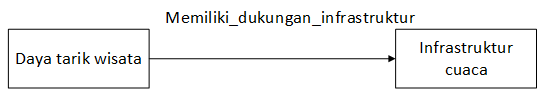
\includegraphics[scale=0.7]{img/rel-diagram.png}
    \caption{diagram relasi daya tarik wisata dengan infrastruktur pendukung cuaca}
    \label{fig:reldiagram}
\end{figure}

Spesifikasi relasi \textbf{memiliki dukungan infrastruktur} dapat dilihat pada tabel \ref{table:hasinssupport}.
\begin{table}[h]
\begin{center}
\begin{tabular}{ |l|m{8cm}| } 
\hline
	\textbf{Spesifikasi} & \textbf{Nilai}\\
	\hline
	Nama relasi & memiliki dukungan infrastruktur\\
	\hline
	Ekuivalen & cuaca cocok\\
	\hline
	Domain konsep & Daya tarik wisata\\
	\hline
	Kardinalitas & (1,1)\\
	\hline
	Target konsep & Infrastruktur cuaca\\
	\hline
\end{tabular}
\end{center}
\caption{Tabel spesifikasi relasi memiliki dukungan infrastruktur}
\label{table:hasinssupport}
\end{table}

Setiap \textit{instance} dari kelas infrastruktur cuaca harus dapat menjabarkan kondisi cuaca apa saja yang direpresentasikan, misalnya cuaca cerah, berawan dsb.
Kondisi cuaca dapat direpresentasikan dengan kode cuaca dari OpenWeatherMap. Kode cuaca dapa dilihat di .Berikut adalah tabel detail dari atribut kode cuaca:
\begin{table}[h]
\begin{center}
\begin{tabular}{ |l|m{8cm}| } 
\hline
	\textbf{Spesifikasi} & \textbf{Keterangan}\\
	\hline
	Nama atribut & kode cuaca\\
	\hline
	Tipe nilai & integer\\
	\hline
	Satuan & --\\
	\hline
	Rentang & [500, 1000]\\
	\hline
\end{tabular}
\end{center}
\caption{Tabel spesifikasi atribut kode cuaca}
\label{table:weatattribute}
\end{table}
\par
Selain kode cuaca, \textit{instance} dari kelas infrastruktur cuaca juga memiliki atribut untuk menyatakan kondisi cuaca menjadi nilai numerik yang dapat digunakan pada proses komputasi.
Hal ini penting pada proses pemberian nilai \textit{utility} daya tarik wisata. Berikut adalah tabel detail dari atribut nilai cuaca:
\begin{table}[h]
\begin{center}
\begin{tabular}{ |l|m{8cm}| } 
\hline
	\textbf{Spesifikasi} & \textbf{Keterangan}\\
	\hline
	Nama atribut & nilai cuaca\\
	\hline
	Tipe nilai & integer\\
	\hline
	Satuan & --\\
	\hline
	Rentang & [1, 3, 5]\\
	\hline
\end{tabular}
\end{center}
\caption{Tabel spesifikasi atribut kode cuaca}
\label{table:weatvalattribute}
\end{table}
\par
Sebagai contoh berikut adalah detail dari salah satu \textit{instance} infrastruktur cuaca, yaitu cuaca bagus.
\begin{table}[h]
\begin{center}
\begin{tabular}{ |l|m{8cm}| } 
\hline
	\textbf{Spesifikasi} & \textbf{Keterangan}\\
	\hline
	Nama instance & \textbf{cuaca bagus} \\
	\hline
	kode cuaca & 801, 802, 803, 804, 952, 953\\
	\hline
	nilai cuaca & 5\\
	\hline
\end{tabular}
\end{center}
\caption{Contoh tabel \textit{instance} daya tarik wisata}
\label{table:instance}
\end{table}


Semua daya tarik wisata pasti memiliki keterangan waktu buka. Setiap hari terdapat perubahan status daya tarik wisata, apakah sedang buka atau sedang tutup.
Karena setiap hari terdapat dua status tersebut dan ada tujuh hari dalam seminggu, maka paling tidak ada empat belas data waktu perubahan status daya tarik wisata.
Tabel \ref{table:timeattribute} adalah contoh spesifikasi atribut waktu perubahan status daya tarik wisata.
 
\begin{table}[h]
\begin{center}
\begin{tabular}{ |l|m{8cm}| } 
\hline
	\textbf{Spesifikasi} & \textbf{Keterangan}\\
	\hline
	Nama atribut & Senin buka\\
	\hline
	Tipe nilai & float\\
	\hline
	Satuan & --\\
	\hline
	Rentang & [0, 1]\\
	\hline
\end{tabular}
\end{center}
\caption{Tabel contoh spesifikasi atribut senin buka}
\label{table:timeattribute}
\end{table}

Nilai yang disimpan pada atribut waktu perubahan status tidak menggunakan format waktu HH:mm, namun dengan nilai \textit{float} antara 0 hingga 1. Hal itu dilakukan
untuk kemudahan proses komputasi dalam pemilihan daya tarik wisata yang sedang buka. Untuk mengkonversi data waktu perubahan status dalam
format HH:mm ke nilai antara nol hingga satu, digunakan persamaan \ref{eq:transform}:

\begin{equation}
tn = \frac{60H + m}{1440}
\label{eq:transform} 
\end{equation}

Dengan $tn$ adalah nilai hasil transformasi ke rentang nol dan satu, $H$ adalah jam dan $m$ adalah menit.
\par
Setiap \textit{instance} daya tarik wisata pasti memiliki atribut \textit{latitude} dan \textit{longitude}, berikut adalah spesifikasi
atribut \textit{latitude} dan \textit{longitude}.
\begin{table}[h]
\begin{center}
\begin{tabular}{ |l|m{8cm}| } 
\hline
	\textbf{Spesifikasi} & \textbf{Keterangan}\\
	\hline
	Nama atribut & latitude \\
	\hline
	Tipe nilai & float\\
	\hline
	Satuan & --\\
	\hline
	Rentang & [-90, 90]\\
	\hline
\end{tabular}
\end{center}
\caption{Tabel spesifikasi atribut latitude}
\label{table:latitude}
\end{table}

\begin{table}[h]
\begin{center}
\begin{tabular}{ |l|m{8cm}| } 
\hline
	\textbf{Spesifikasi} & \textbf{Keterangan}\\
	\hline
	Nama atribut & longitude \\
	\hline
	Tipe nilai & float\\
	\hline
	Satuan & --\\
	\hline
	Rentang & [-180, 180]\\
	\hline
\end{tabular}
\end{center}
\caption{Tabel spesifikasi atribut longitude}
\label{table:longitude}
\end{table}

Spesifikasi relasi dan atribut-atribut yang telah dijabarkan  sebelumnya berfungsi untuk validasi ketika menetapkan nilai-nilai atribut
dan pembuatan relasi pada suatu \textit{instance} daya tarik wisata. Tabel \ref{table:instance} merupakan contoh detail \textit{instance}
daya tarik wisata.
\begin{table}[h]
\begin{center}
\begin{tabular}{ |l|m{8cm}| } 
\hline
	\textbf{Spesifikasi} & \textbf{Keterangan}\\
	\hline
	Nama instance & \textbf{alam wisata cimahi} \\
	\hline
	Latitude & -6.841073f\\
	\hline
	Longitude & 107.54805f\\
	\hline
	Memiliki dukungan infrastruktur & cuaca kurang baik\\
	\hline
	Senin buka & 0.3334f\\
	\hline
	Senin tutup & 0.875f\\
	\hline
	-- & -- \\
	\hline
	Minggu tutup & 0.875f\\
	\hline
\end{tabular}
\end{center}
\caption{Contoh tabel \textit{instance} daya tarik wisata}
\label{table:instance}
\end{table}

\par 
Untuk mendapatkan gambaran jelas dari hubungan antara semantik konsep istilah yang didapatkan, gambar \ref{fig:concept-tree} mmvisualisasikan hubungan tersebut.

\begin{figure}[h!]
    \centering
    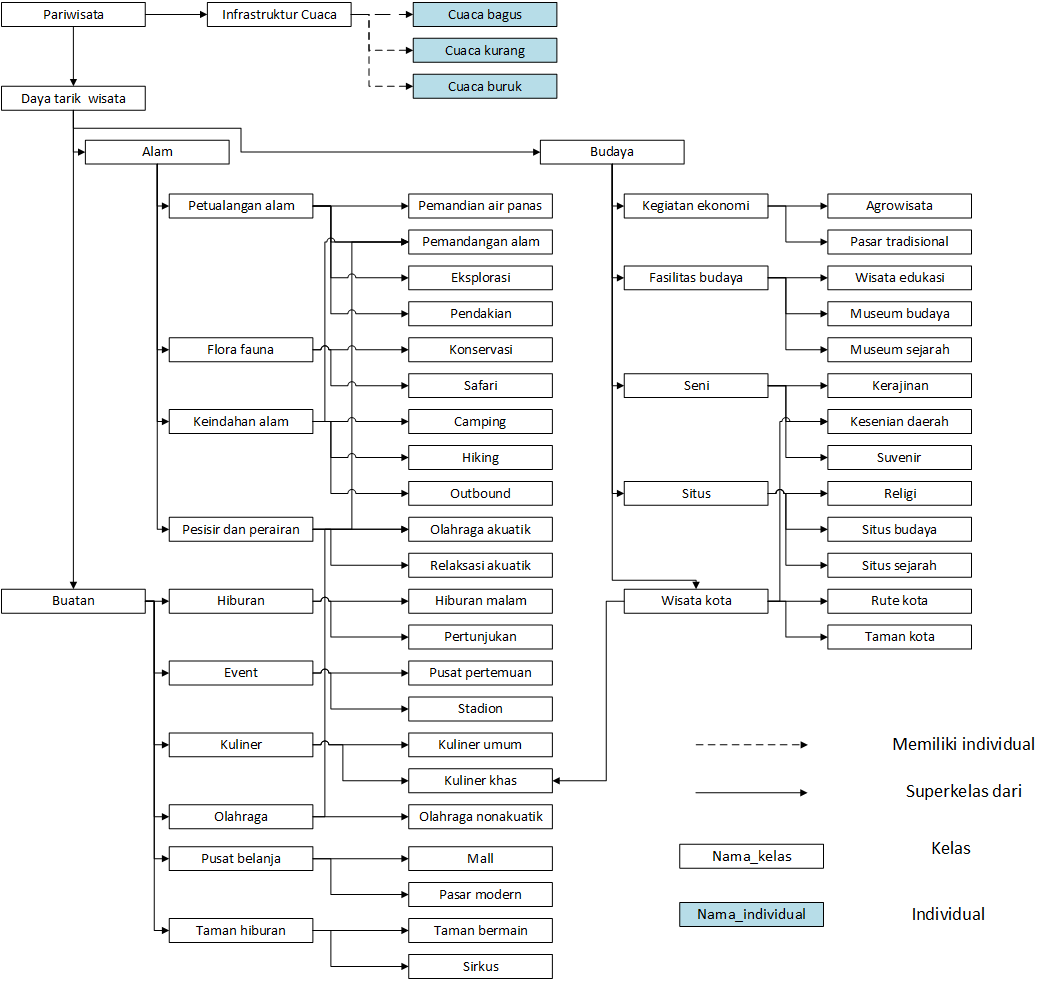
\includegraphics[scale=0.5]{img/concept-tree.png}
    \caption{Gambaran \textit{concept tree} daya tarik wisata}
    \label{fig:concept-tree}
\end{figure}
\cleardoublepage
\subsection{\textit{Knowledge Acquisition}}
\par
Tahap ini merupakan tahap independen dalam pengembangan \textit{ontology}, namun tetap dilaksanakan bersamaan dengan tahap lain.
Untuk domain pariwisata, seabgian besar pengetahuan diperoleh pada awal pengembangan ontology. Ada empat aktivitas yang dilakukan
ketika berada di tahap \textit{knowledge acquisition}, yaitu:
\begin{itemize}
\item Mengadakan wawancara dengan pakar. Wawancara awal ini diadakan dengan tujuan dapat memperoleh ikhtisar dari domain pariwisata.	 
\item Mempelajari literatur yang berhubungan dengan domain pariwisata. Hal ini dapat mengurangi waktu yang diperlukan
dari pakar untuk memberikan instruksi ketika memperoleh konsep domain pariwisata.
\item Setelah memperoleh pengetahuan mengenai domain pariwisata, pencarian konsep bergerak dari umum hingga mengerucut
terutama mengenai kategori daya tarik pariwisata.
\item Konfirmasi konsep domain pariwisata oleh pakar.
\end{itemize}

\subsection{\textit{Implementation}}
\par
Desain \textit{ontology} diimplementsasikan dengan menggunakan \textit{framework} khusus untuk membangun aplikasi
\textit{knowlede-based} yaitu Protege. Protege memiliki beberapa kelebihan, diantaranya: 
\begin{itemize}
\item \textit{Ontology} yang dibangun dengan Protege memenuhi standar W3C,
\item UI sederhana
\item dukungan visualisasi
\end{itemize}

\section{Metodologi Pengembangan Sistem}


Tugas akhir ini akan disusun dengan melalui tahap-tahap berikut:
\begin{enumerate}
\item Pengumpulan Data Lokasi Wisata Bandung
\newline
Tujuan tahap ini adalah mendapatkan data lokasi wisata. Metode yang dapat dilakukan adalah:
\begin{enumerate}
	\item Pencarian data di Google, TripAdvisor dan Foursquare
	\item Pengajuan permintaan data ke Dinas Kebudayaan dan Pariwisata Jawa Barat
\end{enumerate}

\item Analisis Sistem
\par
Beberapa kebutuhan perangkat lunak yang harus dipenuhi dalam membangun \textit{recommender system} ini
adalah:
\begin{enumerate}
	\item Gambaran sistem secara umum
	\item \textit{Graphical user interface}
	\item \textit{Software interface}
	\item Basis data
\end{enumerate}
 
Pada tahap ini juga dilakukan penerapan pengembangan \textit{ontology} dengan \textit{Methontology}.

\item Implementasi Sistem
\newline
Tahap implementasi meliputi:
\begin{enumerate}
	\item Pengembangan aplikasi Android sebagai sisi \textit{client}.
	\item Pengembangan \textit{backend}.
	\item Implementasi komunikasi antara \textit{client} dan \textit{server}. 
	\item Implementasi \textit{ontology} dengan Protege.
\end{enumerate}
 
\item Pengujian
\newline
Tahap pengujian memiliki dua jenis pengujian:
\begin{enumerate}
	\item Pengujian untuk menemukan tingkat kepuasan dari sisi pengguna`
	\item Pengujian akurasi sistem dengan melibatkan pakar. 
\end{enumerate}

\item Pembuatan Laporan
\newline 
Laporan akhir akan ditulis sesuai dengan kaidah dan ketetapan yang berlaku di institusi.
\end{enumerate}


\section{Model Rekomendasi Daya Tarik Wisata}
Sistem yang dikembangkan memiliki masukan berupa prefrensi pengguna terhadap kategori daya tarik wisata tertentu dan 
\textit{contextual factor} seperti lokasi pengguna, cuaca disekitar daya tarik wisata serta waktu lokal. Sistem akan memberikan sepuluh rekomendasi tujuan wisata
paling sesuai berdasarkan masukan yang diterima.

\subsection{Mendapatkan Masukan Preferensi Pengguna}

Untuk mendapatkan preferensi pengguna terhadap suatu kategori daya tarik wisata, pengguna dapat menyatakan secara eksplisit ketertarikan terhadap suatu kategori daya tarik wisata.
Ada empat tingkat ketertarikan pengguna, yaitu tidak ada, rendah, cukup tinggi dan tinggi. Setiap tingkat ketertarikan memiliki nilai bobot tersendiri. Berikut adalah nilai bobot dari
setiap tingkat ketertarikan.
\begin{table}[h]
\begin{center}
\begin{tabular}{ |l|c| } 
\hline
	\textbf{Tingkat} & \textbf{Nilai bobot}\\
	\hline
	Tidak tertarik & 0 \\
	\hline
	Kurang tertarik & 3 \\
	\hline
	Cukup tertarik & 6\\
	\hline
	Sangat tertarik & 9\\
	\hline
\end{tabular}
\end{center}
\caption{Tabel nilai numerik tingkat ketertarikan pengguna terhadap suatu kategori}
\label{table:weight-pref}
\end{table}

Pengguna memilih tingkat ketertarikan yang sesuai melalui tampilan GUI berikut:
\begin{figure}[h!]
    \centering
    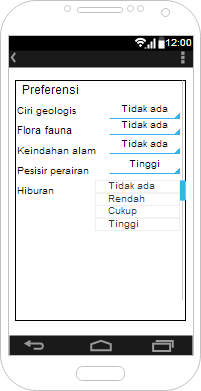
\includegraphics[scale=0.6]{img/gui-pref.png}
    \caption{GUI pada \textit{frontend} untuk mendapatkan masukan tingkat ketertarikan dari pengguna}
    \label{fig:guipref}
\end{figure}
\par
Semua kategori daya tarik wisata merupakan subkelas langsung dari kelas alam, budaya dan buatan. Pengguna dapat mengetahui keterangan kategori daya tarik wisata dengan cara
\textit{tap} teks kategori.

\par
Aplikasi \textit{frontend} akan mengirimkan lokasi dan tingkat ketertarikan pengguna melalui protokol HTTP. Format data yang dikirimkan sebagai HTTP request adalah sebagai
berikut:
\lstset{
   backgroundcolor=\color{white},
   extendedchars=true,
   basicstyle=\footnotesize\ttfamily,
   showstringspaces=false,
   showspaces=false,
   numberstyle=\footnotesize,
   numbersep=9pt,
   tabsize=2,
   breaklines=true,
   showtabs=false,
   captionpos=b
}
\begin{lstlisting}
{	
	"location":{
		"lat":float,
		"lng":float
	},
	"preferences":{
		"Petualangan_alam":int,
		"Flora_fauna":int,
		"Keindahan_alam":int,
		"Pesisir_perairan":int,
		"Hiburan":int,
		"Event":int,
		"Olahraga":int,
		"Pusat_belanja":int,
		"Kuliner":int,
		"Taman_hiburan":int,
		"Kegiatan_ekonomi":int,
		"Fasilitas_budaya":int,
		"Seni":int,
		"Situs":int,
		"Wisata_kota":int
	}
}
\end{lstlisting}

Nilai pada setiap \textit{field} di \textit{preferences} merupakan nilai numerik dari tingkat ketertarikan pengguna terhadap suatu kategori.

\subsection{Menyaring Daya tarik Wisata Berdasarkan Masukan}
\par
Terdapat tiga tahap dalam memproses masukan \textit{recommender system} hingga pengguna mendapat rekomendasi daya tarik wisata. Kedua tahap itu adalah:
\begin{enumerate}
\item \textbf{Memilih daya tarik wisata yang buka}
\par
Untuk memilih daya tarik wisata yang sedang buka, \textit{Context Aware API Server} mengeksekusi SPARQL \textit{query} terhadap objek \textit{ontology}. Sebelum mengeksekusi
\textit{query}, \textit{Context Aware API Server} harus mengetahui jam dan menit saat itu. Kemudian ilai jam dan menit dikonversikan dengan persamaan \ref{eq:transform}.
\par
Seleksi daya tarik wisata dilakukan berdasar atribut waktu perubahan status. Pemilihan atribut dilakukan berdasar hari eksekusi \textit{query}. Berikut adalah contoh 
\textit{query} untuk memilih daya tarik wisata yang sedang buka pada hari senin pukul dua belas siang
\begin{verbatim}
	PREFIX rdf: <http://www.w3.org/1999/02/22-rdf-syntax-ns#>
	PREFIX owl: <http://www.w3.org/2002/07/owl#>
	PREFIX rdfs: <http://www.w3.org/2000/01/rdf-schema#>
	PREFIX xsd: <http://www.w3.org/2001/XMLSchema#>
	PREFIX ns: <http://www.semanticweb.org/dell/ontologies/2017/4/tourism#>
			
	SELECT ?destination 
	WHERE {?destination ns:senin_buka ?open; ns:senin_tutup ?closed 
	FILTER( (?open < 0.5 && 0.5 < ?closed)  
	|| ((?closed > 0.5 || ?open < 0.5) && (?closed < ?open)) )}
\end{verbatim}

Hasil dari \textit{query} diatas adalah daftar nama \textit{instance} daya tarik wisata yang buka hari senin pukul dua belas siang.
\item \textbf{Memberi nilai \textit{utility}}
Nilai \textit{utility} setiap daya tarik wisata ditentukan dengan persamaan berikut:
\begin{equation}
util_i = e^{-(d_i + w_i)} (p_i + 10^{-5})
\label{eq:utility} 
\end{equation}
\par
\textit{Utility} ditentukan dengan fungsi eksponen negatif dari $d_i$ sebagai jarak antara pengguna dengan daya tarik wisata ke $i$, $p_i$ sebagai nilai 
\textit{dissimilarity} antara preferensi pengguna dengan kategori daya tarik wisata ke $i$ dan $w_i$ sebagai selisih nilai cuaca aktual di daya tarik wisata ke $i$ dengan
nilai cuaca yang cocok untuk mengunjungi daya tarik wisata tersebut.Nilai $d_i$ didapatkan dengan persamaan \textit{euclidean}:

\begin{equation}
d_i = \sqrt{(l_1 - x_i)^2 + (l_2 - y_i)^2}
\label{eq:euclidean} 
\end{equation}
\par
dengan $l_1$ adalah \textit{latitude} dan $l_2$ adalah \textit{longitude} pengguna. Sedangkan $x_i$ adalah \textit{latitude} dan $y_i$ adalah \textit{longitude} dari
daya tarik wisata ke $i$.
\par
Sedangkan untuk menghitung nilai \textit{dissimilarity} antara preferensi pengguna terhadap kategori daya tarik wisata ke $i$ dapat menggunakan persamaan \ref{eq:pref}:
\begin{equation}
p_i = -\sum_{j=1}^{|m|} m_j n_{ij}
\label{eq:pref} 
\end{equation}
Sementara $m$ merupakan vektor tingkat ketertarikan pengguna terhadap kategori daya tarik wisata 
dan $n_{ij}$ adalah hubungan antara daya tarik wisata ke $i$ dengan kategori ke $j$. Nilai hubungan tersebut akan selalu bernilai lebih dari sama dengan 0.
\par
Karena setiap daya tarik wisata tidak menjadi \text{instance} langsung dari kategori, melainkan menjadi \text{instance} dari subkategori yang diagregasi oleh suatu kategori,
maka untuk menghitung $n_{ij}$ digunakan persamaan \ref{eq:pref2}:
\begin{equation}
n_{ij} = \sum_{k=1}^{|o|} o_{ik}
\label{eq:pref2} 
\end{equation}
\par
dengan $o_{ik}$ adalah nilai hubungan antara daya tarik wisata ke $i$ dengan subkategori ke $k$ yang menjadi subkelas dari kategori ke $j$. Nilai hubungan menjadi satu jika
\textit{instance} daya tarik wisata memang \textit{instance} dari subkategori tersebut dan nol jika bukan.
\par
Sedangkan untuk menilai seberapa layak daya tarik wisata dikunjungi berdasarkan cuaca menggunakan persamaan \ref{eq:weather}:
\begin{equation}
w_i = s_i - 1
\label{eq:weather} 
\end{equation}
dengan $s_i$ adalah nilai numerik dari kondisi cuaca terkini di daya tarik wisata. Nilai $s_i$
didapatkan dari lokasi acuan cuaca yang paling terdekat dengan daya tarik wisata tersebut.

\end{enumerate}

\section{Desain Sistem}
Sebelum masuk pada fase pengembangan sistem, menentukan desain kasar sistem merupakan hal yang krusial. Hal tersebut disebabkan karena memahami komponen apa saja yang ada pada sistem dan relasi antar komponen dapat membantu menentukan arah pengembangan sistem. 

 
\subsection{Arsitektur Sistem}
\par
Gambar \ref{fig:arch-sys} menjelaskan desain arsitektur sistem dan relasi-relasi antar komponen.
\newline
\begin{figure}[h!]
    \centering
    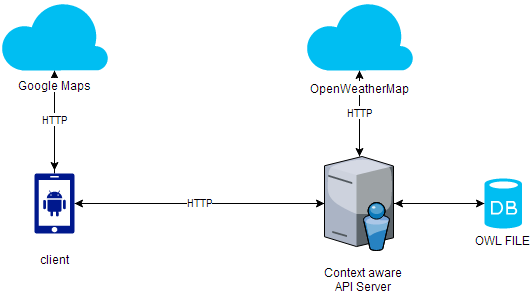
\includegraphics[scale=0.5]{img/arsitektur_sistem.png}
    \caption{Gambaran komponen-komponen sistem dan relasinya}
    \label{fig:arch-sys}
\end{figure}

\par
Terdapat empat lima  komponen penting dari sistem yang dikembangkan, yaitu \textit{client}, \textit{server}, 
\textit{Google Maps API} dan \textit{Open Weather Map API}.

\subsection{Flowchart Sistem}
Secara umum, aliran kerja sistem dijelaskan pada gambar \ref{fig:flowchart} dibawah ini:
\begin{figure}[h!]
    \centering
    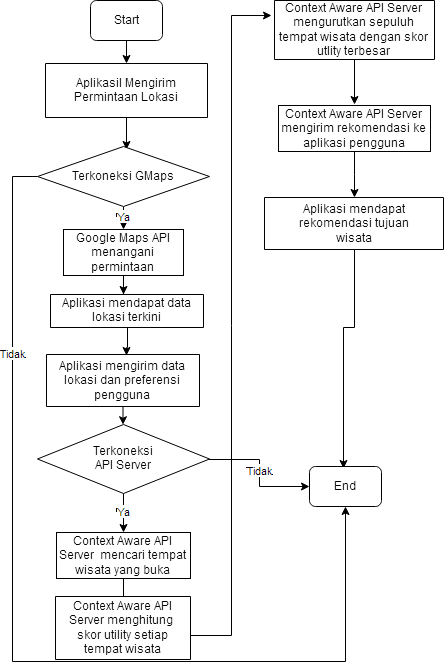
\includegraphics[scale=0.6]{img/flowchart-general.png}
    \caption{Gambaran alur kerja sistem ketika pengguna ingin mendapat rekomendasi daya tarik wisata}
    \label{fig:flowchart}
\end{figure}
\textit{Flowchart} sistem pada gambar \ref{fig:flowchart} dapat dijelaskan secara umum sebagai tiga kegiatan utama. Tiga kegiatan tersebut adalah mendapatkan alur mendapatkan informasi kontekstual dan preferensi tujuan wisata pengguna, 
melakukan \textit{reasoning} di \textit{web server} berdasar data yang masuk, dan mendapatkan rekomendasi tujuan wisata.
\cleardoublepage
\par
\textit{Context Aware API Server} memiliki dua \textit{thread} yang dijalankan bersamaan. \textit{Thread} pertama untuk mendengarkan permintaan rekomendasi tujuan wisata dan yang kedua
untuk memperbaharui data cuaca di lokasi yang menjadi acuan kondisi cuaca.
\begin{figure}[h!]
    \centering
    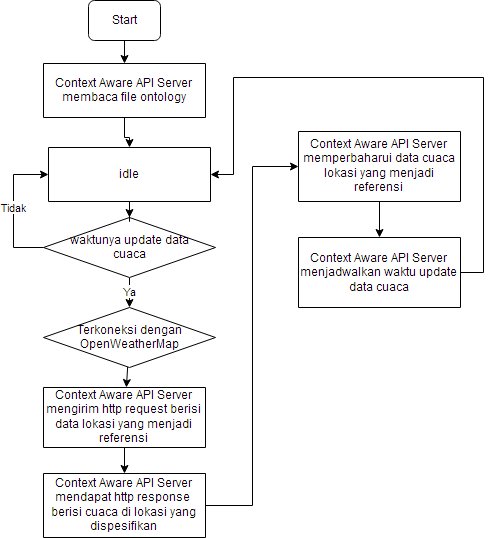
\includegraphics[scale=0.6]{img/flowchart-general-2.png}
    \caption{Gambaran alur kerja sistem aktivitas yang dilakukan server secara berkala}
    \label{fig:flowchart2}
\end{figure}

\section{Skenario Pengujian}
Pengujian dilakukan terhadap pakar pariwisata dan pengguna biasa, sehingga parameter yang diujikan di kedua pengujian pun berbeda.

\subsection{Pengujian dengan Pakar Pariwisata}
\par
Pengujian ini bertujuan untuk mengetahui seberapa besar relevansi rekomendasi yang diberikan kepada pengguna dilihat dari preferensi terhadap
kategori destinasi wisata yang menjadi rekomendasi. Untuk mengukur relevansi rekomendasi, parameter yang dapat digunakan untuk
pengujian adalah \textit{precision}\cite{arnett2015recommender}\cite{chen2012recommendation}.
\textit{Precision} merupakan rasio perbandingan objek yang relevan dengan semua objek yang terpilih. Precision dihitung dengan persamaan \ref{eq:precision}:
\begin{equation}
Precision = \frac{TP}{TP + FP}
\label{eq:precision} 
\end{equation}
\par
dengan $TP$ (\textit{true positive}) adalah destinasi wisata yang tepat dengan preferensi kategori wisata yang dimasukkan dan $FP$ 
(\textit{false positive}) adalah destinasi wisata yang kurang sesuai.

\par
Tabel \ref{table:scenario} adalah skenario pengujian sistem dengan penilaian oleh pakar.
\begin{center}
\small
\begin{longtable}{ |l|l|l|l|m{2cm}| } 
\hline
\textbf{No} & \textbf{Lokasi pengguna} & \textbf{Waktu lokal} & \textbf{Cuaca} & \textbf{No Uji Preferensi} \\
\hline
1	&	Alun-alun Cimahi	&	09:00	& bagus & 1\\
\hline
2	&	Alun-alun Cimahi	&	09:00	& kurang bagus & 1\\
\hline
3	&	Alun-alun Cimahi	&	09:00	& buruk & 1\\
\hline
4	&	Alun-alun Cimahi	&	13:00	& bagus & 2\\
\hline
5	&	Alun-alun Cimahi	&	13:00	& kurang bagus & 2\\
\hline
6	&	Alun-alun Cimahi	&	13:00	& buruk & 2\\
\hline
7	&	Alun-alun Cimahi	&	18:00	& bagus & 3\\
\hline
8	&	Alun-alun Cimahi	&	18:00	& kurang bagus & 3\\
\hline
9	&	Alun-alun Cimahi	&	18:00	& buruk & 3\\
\hline
10	&	Jalan Setiabudhi Bandung	&	09:00	& bagus & 1\\
\hline
11	&	Jalan Setiabudhi Bandung	&	09:00	& kurang bagus & 1\\
\hline
12	&	Jalan Setiabudhi Bandung	&	09:00	& buruk & 1\\
\hline
13	&	Jalan Setiabudhi Bandung	&	13:00	& bagus & 2\\
\hline
14	&	Jalan Setiabudhi Bandung	&	13:00	& kurang bagus & 2\\
\hline
15	&	Jalan Setiabudhi Bandung	&	13:00	& buruk & 2\\
\hline
16	&	Jalan Setiabudhi Bandung	&	18:00	& bagus & 3\\
\hline
17	&	Jalan Setiabudhi Bandung	&	18:00	& kurang bagus & 3\\
\hline
18	&	Jalan Setiabudhi Bandung	&	18:00	& buruk & 3\\
\hline
19	&	Jalan Buah Batu	&	09:00	& bagus & 1\\
\hline
20	&	Jalan Buah Batu	&	09:00	& kurang bagus & 1\\
\hline
21	&	Jalan Buah Batu	&	09:00	& buruk & 1\\
\hline
22	&	Jalan Buah Batu	&	13:00	& bagus & 2\\
\hline
23	&	Jalan Buah Batu	&	13:00	& kurang bagus & 2\\
\hline
24	&	Jalan Buah Batu	&	13:00	& buruk & 2\\
\hline
25	&	Jalan Buah Batu	&	18:00	& bagus & 3\\
\hline
26	&	Jalan Buah Batu	&	18:00	& kurang bagus & 3\\
\hline
27	&	Jalan Buah Batu	&	18:00	& buruk & 3\\
\hline
\caption{Tabel skenario pengujian dengan pakar}
\label{table:scenario}
\end{longtable}
\end{center}

\par
Nomor uji preferensi yang digunakan mengacu pada tabel \ref{table:scenario-pref}:
\begin{center}
\footnotesize
\begin{longtable}{ |l|l|l| } 
\hline
\textbf{No} & \textbf{Kategori Wisata} & \textbf{Tingkat preferensi} \\
\hline
				1	&	Petualangan alam	& Sangat tertarik \\
					&	Flora fauna			& Cukup tertarik \\
					&	Keindahan alam		& Cukup tertarik \\
					&	Pesisir perairan	& Cukup tertarik \\
					&	Hiburan				& Tidak tertarik \\
					&	Event				& Tidak tertarik \\
					&	Olahraga			& Tidak tertarik \\
					&	Pusat belanja		& Tidak tertarik \\
					&	Kuliner				& Tidak tertarik \\
					&	Taman hiburan		& Tidak tertarik \\
					&	Kegiatan ekonomi	& Kurang tertarik \\
					&	Fasilitas budaya	& Tidak tertarik \\
					&	Seni				& Tidak tertarik \\
					&	Situs				& Tidak tertarik \\
					&	Wisata kota			& Tidak tertarik \\
\hline
				2	&	Petualangan alam	& Tidak tertarik \\
					&	Flora fauna			& Tidak tertarik \\
					&	Keindahan alam		& Tidak tertarik \\
					&	Pesisir perairan	& Tidak tertarik \\
					&	Hiburan				& Cukup tertarik \\
					&	Event				& Cukup tertarik \\
					&	Olahraga			& Cukup tertarik \\
					&	Pusat belanja		& Cukup tertarik \\
					&	Kuliner				& Sangat tertarik \\
					&	Taman hiburan		& Sangat tertarik \\
					&	Kegiatan ekonomi	& Tidak tertarik \\
					&	Fasilitas budaya	& Sangat tertarik \\
					&	Seni				& Sangat tertarik \\
					&	Situs				& Sangat tertarik \\
					&	Wisata kota			& Tidak tertarik \\
\hline
				3	&	Petualangan alam	& Tidak tertarik \\
					&	Flora fauna			& Tidak tertarik \\
					&	Keindahan alam		& Tidak tertarik \\
					&	Pesisir perairan	& Tidak tertarik \\
					&	Hiburan				& Sangat tertarik \\
					&	Event				& Tidak tertarik \\
					&	Olahraga			& Cukup tertarik \\
					&	Pusat belanja		& Sangat tertarik \\
					&	Kuliner				& Cukup tertarik \\
					&	Taman hiburan		& Tidak tertarik \\
					&	Kegiatan ekonomi	& Tidak tertarik \\
					&	Fasilitas budaya	& Tidak tertarik \\
					&	Seni				& Cukup tertarik \\
					&	Situs				& Tidak tertarik \\
					&	Wisata kota			& Sangat tertarik \\
\hline
\caption{Tabel uji preferensi}
\label{table:scenario-pref}
\end{longtable}
\end{center}

\subsection{Pengujian dengan Pengguna Umum}
Pengujian terhadap persepsi pengguna umum dilakukan dengan tujuan mendapatkan tingkat akurasi rekomendasi dan tingkat kepuasan pengguna.
Tingkat akurasi rekomendasi yang diperoleh seorang pengguna dihitung dengan persamaan \ref{eq:accuracy}\cite{baizalevaluating}:
\begin{equation}
akurasi = \frac{jumlah\_rekomendasi\_sukses}{jumlah\_permintaan\_rekomendasi}.
\label{eq:accuracy} 
\end{equation}
\par
dengan jumlah rekomendasi sukses bertambah setiap kali pengguna memilih destinasi wisata dari daftar rekomendasi yang baru saja diberikan.
\newline
\par
Untuk mengukur tingkat kepuasan pengguna, parameter evaluasi yang digunakan adalah 
\begin{itemize}
	\item kualitas rekomendasi (\textit{perceived recommendation quality} / PRQ)
	\item kemudahan penggunaan (\textit{usability} / USA) 
	\item seberapa informatif detail destinasi wisata yang direkomendasikan (\textit{informative} / INF)
	\item seberapa efisien aksi yang harus dilakukan pengguna hingga mendapat tujuan wisata yang disukai secara cepat (\textit{perceived efficiency} / PE) 
	\item tingkat kepercayaan pengguna bahwa aplikasi dapat diandalkan untuk memberikan rekomendasi tujuan wisata(\textit{trust} / TR)
\end{itemize}
pengguna akan diminta untuk mengisi kuesioner setelah menggunakan aplikasi minimal satu kali meminta rekomendasi. Pernyataan yang diajukan pada kuesioner adalah sebagai
berikut:

\begin{table}[h]
\begin{center}
\begin{tabular}{ |l|m{8cm}|l| } 
\hline
	\textbf{No} & \textbf{Pernyataan} & \textbf{Parameter}\\
	\hline
	1 & Saya suka dengan tempat wisata yang saya pilih dari daftar rekomendasi & PRQ \\
	\hline
	2 & Saya suka interaksi aplikasi ini & PRQ \\
	\hline
	3 & Saya merasa deskripsi tempat wisata di daftar rekomendasi sudah cukup informatif & INF \\
	\hline
	4 & Saya memiliki kesulitan dalam menggunakan aplikasi ini & USA \\
	\hline
	5 & Saya dapat menemukan tujuan wisata yang saya suka secara cepat & PE \\
	\hline
	6 & Saya akan menggunakan aplikasi ini jika saya ingin berwisata di Bandung & TR \\
	\hline
\end{tabular}
\end{center}
\caption{Tabel pertanyaan kuesioner}
\label{table:questionnaire}
\end{table}

Model dan pernyataan kuesioner yang disebutkan pada tabel \ref{table:questionnaire} diambil dari studi sebelumnya yang juga membahas
evaluasi \textit{recommender system}\cite{baizalevaluating}. 
%
%\chapter{Hasil dan Pembahasan}

\par
Pengujian dilakukan dengan pakar dan pengguna biasa, sehingga skenario pengujian pun berbeda.
\section{Hasil Pengujian dengan Pakar Pariwisata}

\par
Dengan menggunakan skenario \ref{table:scenario}, berikut adalah hasil yang didapatkan dari pengujian dengan pakar:
\begin{center}
\small
\begin{longtable}{ |l|l|l|l|l|l| } 
\hline
\textbf{No} & \textbf{Lokasi pengguna} & \textbf{Waktu} & \textbf{Cuaca} & \textbf{No Uji} & \textbf{Presisi}\\
\hline
1	&	Alun-alun Cimahi	&	09:00	& bagus & 1 & 1\\
\hline
2	&	Alun-alun Cimahi	&	09:00	& kurang bagus & 1 & 1\\
\hline
3	&	Alun-alun Cimahi	&	09:00	& buruk & 1 & 1\\
\hline
4	&	Alun-alun Cimahi	&	13:00	& bagus & 2 & 1\\
\hline
5	&	Alun-alun Cimahi	&	13:00	& kurang bagus & 2 & 1\\
\hline
6	&	Alun-alun Cimahi	&	13:00	& buruk & 2 & 0.9\\
\hline
7	&	Alun-alun Cimahi	&	18:00	& bagus & 3 & 1\\
\hline
8	&	Alun-alun Cimahi	&	18:00	& kurang bagus & 3 & 1\\
\hline
9	&	Alun-alun Cimahi	&	18:00	& buruk & 3 & 0.7\\
\hline
10	&	Jalan Setiabudhi Bandung	&	09:00	& bagus & 1 & 1\\
\hline
11	&	Jalan Setiabudhi Bandung	&	09:00	& kurang bagus & 1 & 1 \\
\hline
12	&	Jalan Setiabudhi Bandung	&	09:00	& buruk & 1 & 0.9\\
\hline
13	&	Jalan Setiabudhi Bandung	&	13:00	& bagus & 2 & 1\\
\hline
14	&	Jalan Setiabudhi Bandung	&	13:00	& kurang bagus & 2 & 1\\
\hline
15	&	Jalan Setiabudhi Bandung	&	13:00	& buruk & 2 & 0.9\\
\hline
16	&	Jalan Setiabudhi Bandung	&	18:00	& bagus & 3 & 1\\
\hline
17	&	Jalan Setiabudhi Bandung	&	18:00	& kurang bagus & 3 & 0.9\\
\hline
18	&	Jalan Setiabudhi Bandung	&	18:00	& buruk & 3 & 0.7\\
\hline
19	&	Jalan Buah Batu	&	09:00	& bagus & 1 & 1\\
\hline
20	&	Jalan Buah Batu	&	09:00	& kurang bagus & 1 & 1\\
\hline
21	&	Jalan Buah Batu	&	09:00	& buruk & 1 & 0.9\\
\hline
22	&	Jalan Buah Batu	&	13:00	& bagus & 2 & 1\\
\hline
23	&	Jalan Buah Batu	&	13:00	& kurang bagus & 2 & 1\\
\hline
24	&	Jalan Buah Batu	&	13:00	& buruk & 2 & 0.8\\
\hline
25	&	Jalan Buah Batu	&	18:00	& bagus & 3 & 1\\
\hline
26	&	Jalan Buah Batu	&	18:00	& kurang bagus & 3 & 0.8\\
\hline
27	&	Jalan Buah Batu	&	18:00	& buruk & 3 & 0.6\\
\hline
\caption{Tabel skenario pengujian dengan pakar}
\label{table:result-1}
\end{longtable}
\end{center}

\begin{figure}[h!]
    \centering
    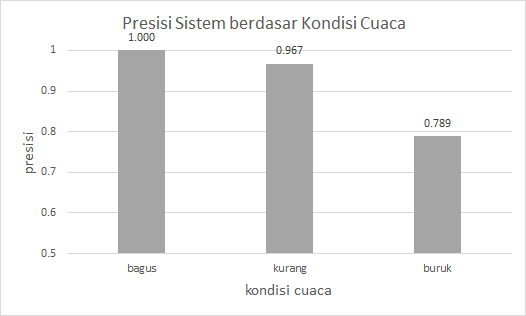
\includegraphics[scale=0.7]{img/precision_weather.png}
    \caption{Mean presisi sistem berdasar kondisi cuaca}
    \label{fig:p_weather}
\end{figure}


\begin{figure}[h!]
    \centering
    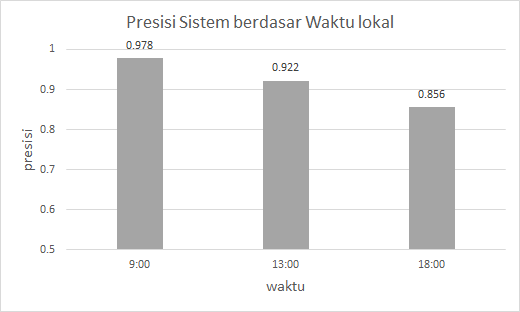
\includegraphics[scale=0.7]{img/precision_time.png}
    \caption{Mean presisi sistem berdasar waktu lokal pengujian}
    \label{fig:p_time}
\end{figure}

\section{Hasil Pengujian dengan Pengguna Biasa}
\begin{figure}[h!]
    \centering
    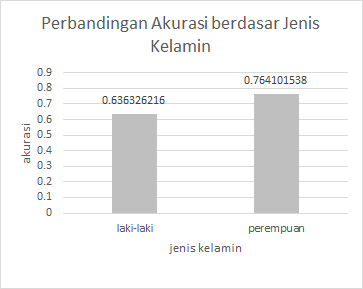
\includegraphics[scale=1]{img/accuracy-gender.png}
    \caption{Akurasi sistem berdasar jenis kelamin}
    \label{fig:accuracy-gender}
\end{figure}

\begin{figure}[h!]
    \centering
    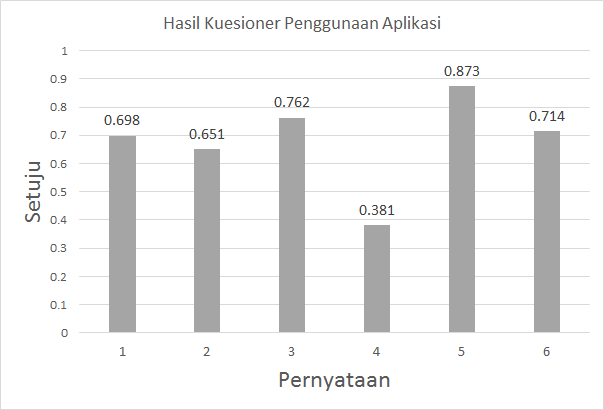
\includegraphics[scale=0.7]{img/hasil_kuesioner.png}
    \caption{Hasil kuesioner pengguna aplikasi}
    \label{fig:quest}
\end{figure}
%
%\chapter{Kesimpulan}
\section{Kesimpulan}
\begin{enumerate}
	\item Presisi rekomendasi destinasi wisata menjadi turun jika sistem digunakan pada malam hari. 
	
\end{enumerate}
\section{Saran}
\par
Berikut adalah saran mengenai hal-hal yang bisa dikembangkan dari tugas akhir ini:
\begin{enumerate}
	\item Menambah masukan \textit{contextual factor} seperti suasana hati pengguna dan keramaian jalan menuju destinasi wisata.
	\item Menggunakan \textit{navigation by proposing} yang digabung dengan \textit{contexttual factor} sehingga sistem lebih intuitif
	dengan masukan pengguna.
\end{enumerate}

%
\cleardoublepage
\addcontentsline{toc}{chapter}{Daftar Pustaka}
\bibliographystyle{acm} %harvard style
\bibliography{References.bib}
%
%\pagebreak
\cleardoublepage
\addcontentsline{toc}{chapter}{Lampiran}
\chapter*{Lampiran}

\end{document}
